% !TeX spellcheck = de_DE/GB

\chapter{Weitere Hardware}
In den nachfolgenden Kapiteln folgt eine Aufzählung und Erläuterung der wesentlichen, zusätzlich benötigten Hardware. Dazu zählen Aktoren zur Darstellung des Betriebszustandes, Schalter und weitere Komponente, die für den Aufbau des Schrittmotor-Demonstrators nötig waren.  

\section{LC-Display-Modul}
Zur Feststellung des aktuellen Betriebszustandes und zur Ausgabe des eingestellten Verfahrweges des Schlittens dient ein Liquid Crystal Display (LC-Display). LC-Displays nutzen ein passives Anzeigetechnologie, denn sie emittieren selbst kein Licht, stattdessen nutzen sie das Umgebungslicht, hier in Form einer 5 V LED. Dadurch sind sie sehr Verbrauchsarm und können relativ kompakt gebaut werden.\cite{HTech.2015} Insgesamt ist das Modul 80 mm x 36 mm groß mit einer Displaygröße von 73,8 mm x 27,1 mm (3 Zoll). Auf dem Display können zeitgleich 16 Zeichen pro Zeile auf insgesamt 2 Zeilen angezeigt werden. Der beste Betrachtungswinkel ist von unten nach oben und das Blickfeld ist in der Frontansicht 60 Grad groß. Bei größeren Abständen wird das Bild zunehmend schlechter, dies ist jedoch für dieses Projekt völlig ausreichend. Zur Stromversorgung wird 5 V Gleichstromspannung benötigt. Mithilfe von 4 Steckbrückenkabel ist es mit dem Arduino verbunden, um es mit der nötigen Spannung zu versorgen und die I2C Verbindung herzustellen (Verdrahtung detailliert in Kapitel XX). Die zur I2C-Kommunikation nötige Adresse ist 0x3F. %oder 0x27 (je nach Chip)
Zusätzliche Spezifikationen des Displays sind: 
	\begin{itemize}
		\item I2C-Kommunikationsschnittstelle 
		\item Kontraststeuerung
		\item blaue Hintergrundbeleuchtung mit weißer Schrift
	\end{itemize}
\cite{WaveShare.2007}

\section{Signalleuchte}
Zusätzlich zum LC-Display ist eine SMD-LED-Signalleuchte zur Zustandserkennung verbaut. Sie soll Störungen und Fehler erkenntlich machen. SMD steht für \emph{Surface Mount Device} und bedeutet, dass die Signalleuchte für Oberflächenmontagen konzipiert ist. Die Leuchte ist dabei mit einem einfachen Stecksystem am Gehäuse befestigt. Dazu wird sie in einer 8 mm Montagebohrung des Gehäuses gesteckt und über die 10 mm Gehäuseblende der Signalleuchte fixiert. Die Leuchte hat eine 3 mm Durchmesser große LED und emittiert ein rotes Licht. Die Betriebsspannung liegt zwischen 2 bis 2,4 V und der Betriebsstrom bei 20 mA. Angeschlossen wird sie über vier Litzen am Arduino (verweis auf Schaltplan).\cite{Mentor.2024}

\section{Spannungswandler}
Für den Aufbau des Demonstrators sind mehrere Spannungswandler nötig. Zum einen ist ein Wechselspannung/Gleichspannungswandler (AD/DC Wandler) in Form des Schaltnetzteils SNT RD 50A eingesetzt. 

\section{Linearführung}
Zur Demonstration einer linearen Bewegung wird eine kompakte Linearführung verwendet. Die Führung ist 400 mm lang und 12 mm breit. Diese Linearführung wird vor allem in Fused Deposition Modeling (FDM) -Drucker verwendet, wo es auf hohe Präzision bei niedrigen Toleranzen ankommt. Deshalb eignet sich diese Führung auch gut für dieses Projekt, wo es nicht darum geht, große Lasten zu Bewegen, sondern möglichst genau die Schrittauflösung auf eine Millimeterskala zu übertragen.
%Von dem Kaufteil gibt es kein Datenblatt

\section{Drehwinkel-Encoder}
Der Demonstrator soll mehrere Programme fahren können, deswegen wurde ein Drehwinkel-Encoder der Steuerung hinzugefügt. Dieser wird über fünf Pins am Arduino angeschlossen. Durch drehen des Drehschalters werden nacheinander zwei Kontakte geschlossen oder geöffnet. Dieser dadurch entstehende Signalfluss, bestehend aus zwei um 90 Grad versetzte Sinus bzw. Cosinus Schwingungen werden ausgewertet. Daraus wird bestimmt, in welcher Richtung (im oder gegen Uhrzeigersinn) und wie weit (inkrementell) gedreht wurde. Mithilfe dieser Logik kann ein Wert erzeugt und eingegeben werden, die der Schrittmotor fahren soll.\cite{Basler.2016} Bei einer Drehung im Uhrzeigersinn wird ein positiver Wert in Millimeter erzeugt und bei einer Drehung gegen den Uhrzeigersinn wird dieser Wert verringert. Zusätzlich zum Drehwinkel-Encoder ist auch noch ein Schaltfunktion im Bauteil selbst integriert. Durch eindrücken des Encoders wird ein Taster betätigt, durch denn der eingestellte Wert bestätigt und an den Arduino zur weiteren Verarbeitung weitergegeben wird. Zur Besseren Handhabung des Drehwinkel-Encoders wurde noch ein Drehgriff angefertigt und auf dem Drehgeber montiert.
Weitere Details: \begin{itemize}
	\item \textbf{Abmessungen (b x l x h):} 18 mm x 31 mm x 30 mm
	\item \textbf{Betriebsspannung:} 3,3 V - 5 V
	\cite{SimacElec.2019}
	
\section{Materialliste}
Alle weiteren im Projekt verwendeten Komponenten können der Materialliste entnommen werden.
	\begin{center}
		\fontsize{8}{10}\selectfont
		\begin{tabularx}{\textwidth}{|p{0.4cm}|p{0.4cm}|X|X|p{1cm}|X|}
			\hline 
			\textbf{Pos.} & \textbf{Stk.} & \textbf{Bezeichnung} & \textbf{Artikel-Nr.} & \textbf{Preis[€]} & \textbf{Bestelladresse} \\ \hline
			1 & 1 & Arduino Lern-Kit: & ARD KIT TINYML & 52,40 & \href{https://www.reichelt.de}{www.reichelt.de} \\
			&   & - Arduino Nano Sense BLE 33 BLE Lite & & & \\ 
			&   &- USB-A-Micro Verbindungskabel & & & \\
			&   &- Klemmboard & & & \\
			\hline
			2 & 1 & CR-10 Nema 17 Schrittmotor 34mm 42-34 & RBS12536 & 14,25 & \href{https://www.roboter-bausatz.de/p/cr-10-nema-17-schrittmotor-34mm-42-34}{www.roboter-bausatz.de} \\
			\hline
			
			3 & 1 & 1 Meter Aluprofil 20x20 I-Typ Nut 5 & RBS12105 & 11,81 & \href{https://www.roboter-bausatz.de/p/1-meter-aluprofil-20x20-i-typ-nut-5}{www.roboter-bausatz.de} \\ 
			\hline
			4 & 1 & Schaltnetzteil, geschlossen, 50 W, 5 / 12 V, 6 A & SNT RD 50A
			& 17,10 & \href{https://www.reichelt.de}{www.reichelt.de} \\ 
			\hline
			5 & 1 & Spannungswandler Power Adapter Modul 12V auf 3.3V/5V/12V AMS1117
			& RBS16534 & 1,68 & \href{https://www.roboter-bausatz.de/p/spannungswandler-power-adapter-modul-12v-auf-3.3v-5v-12v-ams1117}{www.roboter-bausatz.de} \\ 
			\hline
			6 & 1 & GT2 Riemenscheibe 20 Zähne 5mm Bohrung für 6mm Riemen & RBS10277 & 1,15 & \href{https://www.roboter-bausatz.de/p/gt2-riemenscheibe-20-zaehne-5mm-bohrung-fuer-6mm-riemen}{www.roboter-bausatz.de} \\ 
			\hline
			7 & 1 & GT2 Riemenscheibe 20 Zähne 5mm Bohrung mit Dual Kugellager & RBS12569 & 1,85 &	\href{https://www.roboter-bausatz.de/p/gt2-riemenscheibe-20-zaehne-5mm-bohrung-mit-dual-kugellager}{www.roboter-bausatz.de} \\ 
			\hline
			8 & 1 & yourDroid PLA Filament Grau 1.75mm 1kg  & RBS13428 & 15,70 & \href{https://www.roboter-bausatz.de/p/yourdroid-pla-filament-grau-1.75mm-1kg}{www.roboter-bausatz.de} \\ 
			\hline
			9 & 1 & Linearführung MGN12H 450mm & RBS12916 & 32,86 & \href{https://www.roboter-bausatz.de/p/linearfuehrung-mgn12h-450mm}{www.roboter-bausatz.de} \\
			\hline
			10 & 1 & yourDroid GT2 Zahnriemen offen 6mm 1 Meter faserverstärkt & RBS10161 & 2,79 & \href{https://www.roboter-bausatz.de/p/yourdroid-gt2-zahnriemen-offen-6mm-1-meter-faserverstaerkt}{www.roboter-bausatz.de} \\
			\hline
			11 & 30 & M3 Hammermutter T-Schlitz Nut 6 &  RBS11229 & 0,25 & \href{https://www.roboter-bausatz.de/p/m3-hammermutter-t-schlitz-nut-6}{www.roboter-bausatz.de} \\
			\hline
			12 & 30 & M3x20mm Sechskantschraube DIN912 Edelstahl & RBS14063 & 0,10 &
			\href{https://www.roboter-bausatz.de/p/m3x20mm-sechskantschraube-din912-edelstahl}{www.roboter-bausatz.de} \\
			\hline
			13 & 1 & BMI Lineal 963050030 Maßstab 0.5 m Edelstahl & 823983 - 62 & 9,49 & \href{https://www.conrad.de/}{www.conrad.de} \\
			\hline
			14 & 1 & 65 Jumper Wire Kabel im Set & RBS10023 & 1,59 & \href{https://www.roboter-bausatz.de/p/65-jumper-wire-kabel-im-set}{www.roboter-bausatz.de} \\
			\hline
			15 & 1 & 40 Pin Dupont / Jumper Kabel Buchse-Buchse 20 cm & RBS101136 & 1,09 & \href{https://www.roboter-bausatz.de/p/40-pin-dupont-jumper-kabel-buchse-buchse-20-cm}{www.roboter-bausatz.de} \\
			\hline
			16 & 1 & Netzkabel mit Schuko-Stecker 3-adrig offenes Ende 2m & RBS14326 & 5,12 & \href{https://www.roboter-bausatz.de/p/netzkabel-mit-schuko-stecker-3-adrig-offenes-ende-2m}{www.roboter-bausatz.de} \\
			\hline
			17 & 1 & Wippschalter Ein / Aus 250V 6A (rot) & RBS11439 & 0,55 & \href{https://www.roboter-bausatz.de/p/wippschalter-ein-aus-250v-6a-rot}{www.roboter-bausatz.de} \\
			\hline
			18 & 1 & Entwicklerboards - Drehwinkel-Encoder & KY-040 & 2,20 & \href{www.reichelt.de}{www.reichelt.de} \\
			\hline
			19 & 1 & Kontermutter für Potentiometerknöpfe & P4-Mutter & 0,22 & \href{www.reichelt.de}{www.reichelt.de} \\
			\hline
			20 & 1 & Drucktaster Button Schalter Grün 12mm 250V 1A  & RBS13869 & 0,85 & \href{https://www.roboter-bausatz.de/p/drucktaster-button-schalter-gruen-12mm-250v-1a}{www.roboter-bausatz.de} \\
			\hline
			21 & 1 & Mikroschalter / Miniatur Endschalter & RBS 10856 & 0,49 & \href{https://www.roboter-bausatz.de/p/mikroschalter-miniatur-endschalter}{www.roboter-bausatz.de} \\
			\hline
			22 & 1 & Entwicklerboards - Schrittmotorsteuerung, A4988 & DEBO DRV A4988 & 5,80 & \href{https://wwww.reichelt.de}{www.reichelt.de} \\
			\hline
		\end{tabularx}
		\newpage
		\fontsize{8}{10}\selectfont
		\begin{tabularx}{\textwidth}{|p{0.4cm}|p{0.4cm}|X|X|p{1cm}|X|}
			\hline 
			\textbf{Pos.} & \textbf{Stk.} & \textbf{Bezeichnung} & \textbf{Artikel-Nr.} & \textbf{Preis[€]} & \textbf{Bestelladresse} \\ \hline
			23 & 2 & JST - Buchsengehäuse, 1x4-polig - EH & JST EH4P BU & 0,09 & \href{https://wwww.reichelt.de}{www.reichelt.de} \\
			\hline
			24 & 1 & Signallleuchte, SMD-LED, ø3mm, Kunststoff & MEN 2660.8301 & 4,60 & \href{https://wwww.reichelt.de}{www.reichelt.de} \\
			\hline
			25 & 1 & LCD Display Modul 1602 HD44780 I2C (gelötet) & RBS15585 & 4,45 & \href{https://www.roboter-bausatz.de/p/lcd-display-modul-1602-hd44780-i2c-geloetet}{www.roboter-bausatz.de} \\
			\hline
			26 & 1 & Einpressmuttern M3x4x4 100 Stück für Voron 2.4 & RBS15553 & 3,14 & \href{https://www.roboter-bausatz.de/p/einpressmuttern-m3x4x4-100-stueck-fuer-voron-2.4}{www.roboter-bausatz.de} \\
			\hline
		\end{tabularx}
		
		\captionof{table}{Materialliste}
	\end{center}
	
\end{itemize}
\section{Schaltplan}
\begin{figure}[htb]
	\begin{center}
		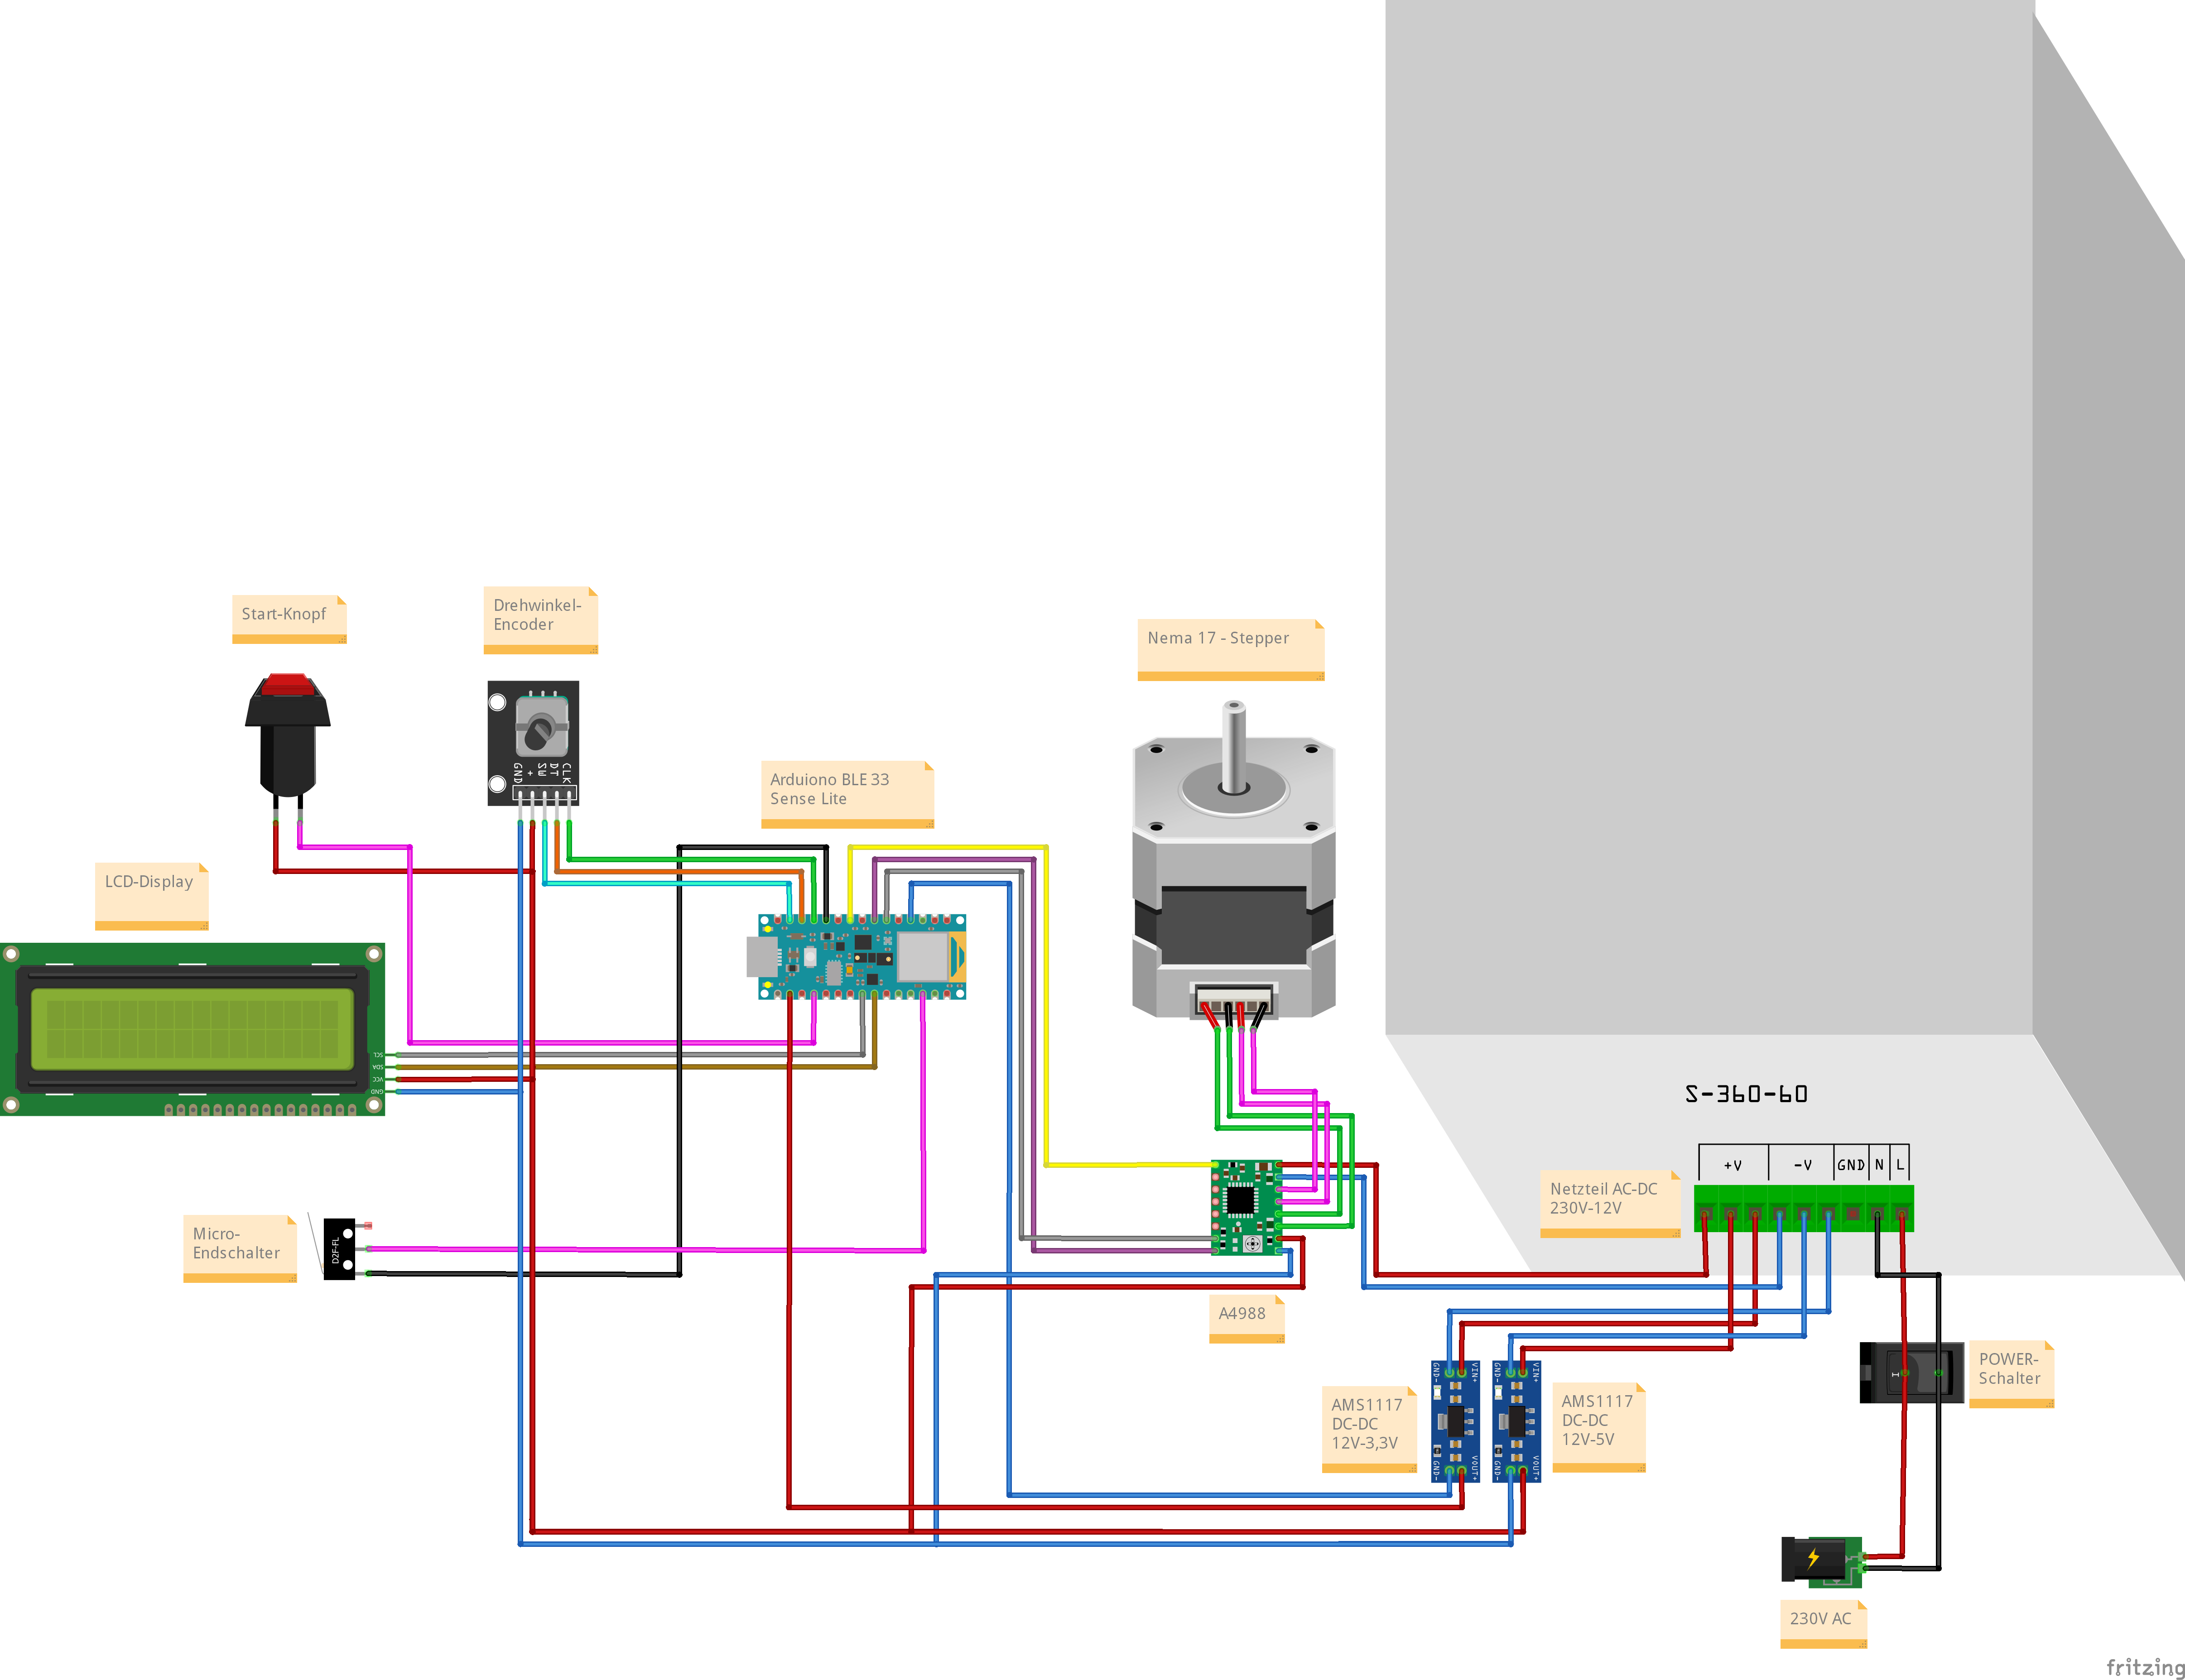
\includegraphics[width=\textwidth]{Images/Schaltplan1.png}
		\caption{Schaltplan} \label{Schaltplan}
	\end{center}
\end{figure}





